%%%%%%%%%%%%%%%%%%%%%%%%%%%%%%%%%%%%

\section{Point estimates and sampling variability!!!}

%%%%%%%%%%%%%%%%%%%%%%%%%%%%%%%%%%%%

\subsection{Point estimates and error}

%%%%%%%%%%%%%%%%%%%%%%%%%%%%%%%%%%%%

\begin{frame}
\frametitle{Point estimates and error}

\begin{itemize}

\item We are often interested in \hl{population parameters}.

\item Complete populations are difficult to collect data on, so we use \hl{sample statistics} as \hl{point estimates} for the unknown population parameters of interest.

\item \hl{Error} in the estimate = difference between population parameter and sample statistic

\item \hl{Bias} is systematic tendency to over- or under-estimate the true population parameter.

\item \hl{Sampling error} describes how much an estimate will tend to vary from one sample to the next.

\item Much of statistics is focused on understanding and quantifying sampling error, and \hl{sample size} is helpful for quantifying this error.

\end{itemize}

\end{frame}

%%%%%%%%%%%%%%%%%%%%%%%%%%%%%%%%%%%

\begin{frame}
\frametitle{}

\dq{Suppose we randomly sample 1,000 adults from each state in the US. Would you expect the sample means of their heights to be the same, somewhat different, or very different?}

\pause

\soln{Not the same, but only somewhat different.}

\end{frame}

%%%%%%%%%%%%%%%%%%%%%%%%%%%%%%%%%%%%

\subsection{Understanding the variability of a point estimate}

%%%%%%%%%%%%%%%%%%%%%%%%%%%%%%%%%%%%

\begin{frame}
\frametitle{}

\begin{center}
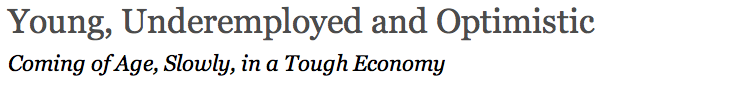
\includegraphics[width=0.95\textwidth]{\chp5@path/5-1_point_est_sampling_var/figures/pew/pew1} \\
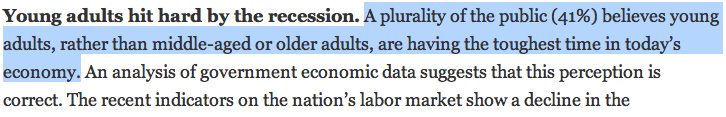
\includegraphics[width=0.95\textwidth]{\chp5@path/5-1_point_est_sampling_var/figures/pew/pew2} \\
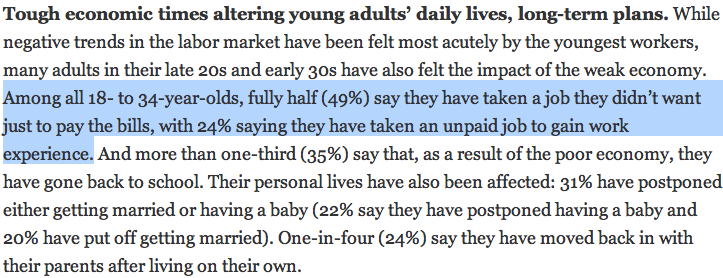
\includegraphics[width=0.95\textwidth]{\chp5@path/5-1_point_est_sampling_var/figures/pew/pew3}
\end{center}

\ct{\webURL{http://pewresearch.org/pubs/2191/young-adults-workers-labor-market-pay-careers-advancement-recession}}

\end{frame}

%%%%%%%%%%%%%%%%%%%%%%%%%%%%%%%%%%%%

\begin{frame}
\frametitle{Margin of error}

\begin{center}
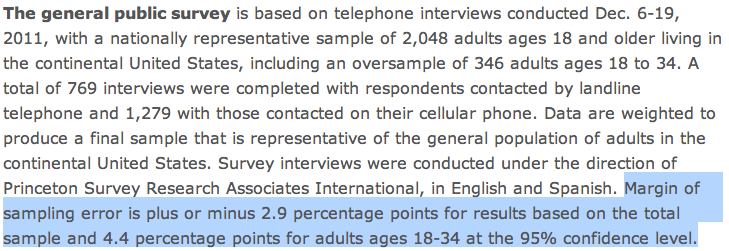
\includegraphics[width=0.95\textwidth]{\chp5@path/5-1_point_est_sampling_var/figures/pew/pew4}
\end{center}

\begin{itemize}

\item 41\% $\pm$ 2.9\%: We are 95\% confident that 38.1\% to 43.9\% of the public believe young adults, rather than middle-aged or older adults, are having the toughest time in today's economy.

\item 49\% $\pm$ 4.4\%: We are 95\% confident that 44.6\% to 53.4\% of 18-34 years olds have taken a job they didn't want just to pay the bills.

\end{itemize}

\end{frame}

%%%%%%%%%%%%%%%%%%%%%%%%%%%%%%%%%%%

\subsection{Application exercise}

%%%%%%%%%%%%%%%%%%%%%%%%%%%%%%%%%%%

\begin{frame}
\frametitle{}

\dq{Suppose the proportion of American adults who support the expansion of solar energy is p = 0.88, which is our parameter of interest. Is a randomly selected American adult more or less likely to support the expansion of solar energy?}

\pause

\soln{More likely.}

\end{frame}

%%%%%%%%%%%%%%%%%%%%%%%%%%%%%%%%

\begin{frame}
\frametitle{}

\dq{Suppose that you don't have access to the populaion of all American adults, which is a quite likely scenario. In order to estimate the proportion of American adults who support solar power expansion, you might sample from the population and use your sample proportion as the best guess for the unknown population proportion.}

\begin{itemize}

\item Sample, with replacement, 1000 American adults from the population, and record whether they support or not solar power expansion.

\item Find the sample proportion.

\item Plot the distribution of the sample proportions obtained by members of the class.

\end{itemize}

\end{frame}

%%%%%%%%%%%%%%%%%%%%%%%%%%%%%%%%%%%

\begin{frame}[fragile]
\frametitle{}

\begin{beamerboxesrounded}[shadow = true, lower = code body]{}
{
\small 
\begin{verbatim}

# 1. Create a set of 250 million entries, where 88\% of 
# them are "support" and 12\% are "not".

pop_size <- 250000000
possible_entries <- c(rep("support", 0.88 * pop_size), 
                      rep("not", 0.12 * pop_size))


# 2. Sample 1000 entries without replacement.

sampled_entries <- sample(possible_entries, size = 1000)

# 3. Compute p-hat: count the number that are "support", 
# then divide by # the sample size.

sum(sampled sampled_entries == "support") / 1000

\end{verbatim}
}
\end{beamerboxesrounded}

\end{frame}

%%%%%%%%%%%%%%%%%%%%%%%%%%%%%%%%%%%

\begin{frame}
\frametitle{Sampling distribution}

Suppose you were to repeat this process many times and obtain many $\hat{p}$s. This distribution is called a \hl{sampling distribution}.

\begin{center}
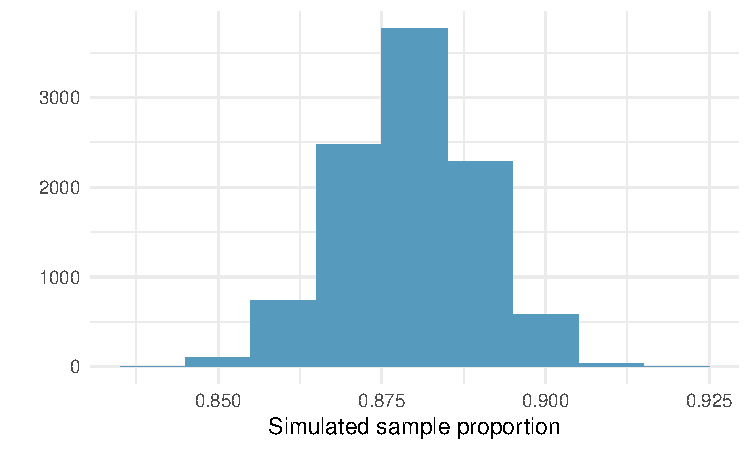
\includegraphics[width=0.6\textwidth]{\chp5@path/5-1_point_est_sampling_var/figures/solar-power/solar-power-sampling.pdf}
\end{center}

\end{frame}

%%%%%%%%%%%%%%%%%%%%%%%%%%%%%%%%%%%

\begin{frame}
\frametitle{}

\dq{What is the shape and center of this distribution? Based on this distribution, what do you think is the true population proportion?}

\begin{center}
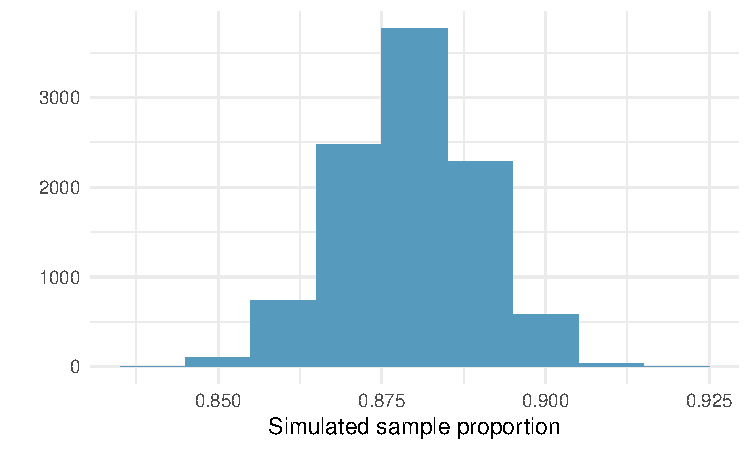
\includegraphics[width=0.6\textwidth]{\chp5@path/5-1_point_est_sampling_var/figures/solar-power/solar-power-sampling.pdf}
\end{center}

$\:$ \\
\soln{\only<2>{
The distribution is unimodal and roughly symmetric. A reasonable guess for the true population proportion is the center of this distribution, approximately 0.88.
}}

\end{frame}

%%%%%%%%%%%%%%%%%%%%%%%%%%%%%%%%

\begin{frame}
\frametitle{Sampling distributions are never observed}

\begin{itemize}

\item In real-world applications, we never actually observe the sampling distribution, yet it is useful to always think of a point estimate as coming from such a hypothetical distribution.

\item Understanding the sampling distribution will help us characterize and make sense of the point estimates that we do observe.

\end{itemize}

\end{frame}

%%%%%%%%%%%%%%%%%%%%%%%%%%%%%%%%

\subsection{Central Limit Theorem}

%%%%%%%%%%%%%%%%%%%%%%%%%%%%%%%%%%

\begin{frame}
\frametitle{Central Limit Theorem}

\formula{Central limit theorem}
{Sample proportions will be nearly normally distributed with mean equal to the population proportion, $p$, and standard error equal to $\sqrt{\frac{p~(1-p)}{n}}$.
\[ \hat{p} \sim N \pr{ mean = p, SE = \sqrt{\frac{p~(1-p)}{n}} } \]
}

\begin{itemize}

\item It wasn't a coincidence that the sampling distribution we saw earlier was symmetric, and centered at the true population proportion.

\item We won't go through a detailed proof of why $SE =  \sqrt{\frac{p~(1-p)}{n}}$, but note that as $n$ increases $SE$ decreases.
\begin{itemize}
\item As $n$ increases samples will yield more consistent $\hat{p}$s, i.e. variability among $\hat{p}$s will be lower.
\end{itemize}

\end{itemize}

\end{frame}

%%%%%%%%%%%%%%%%%%%%%%%%%%%%%%%%%%%%

\begin{frame}
\frametitle{CLT - conditions}

Certain conditions must be met for the CLT to apply:

\begin{enumerate}

\item \hlGr{Independence:} Sampled observations must be independent. \\

This is difficult to verify, but is more likely if
\begin{itemize}
\item random sampling/assignment is used, and
\item if sampling without replacement, $n$ $<$ 10\% of the population.
\end{itemize}

\pause

\item \hlGr{Sample size:} There should be at least 10 expected successes and 10 expected failures in the observed sample.

This is difficult to verify if you don't know the population proportion (or can't assume a value for it). In those cases we look for the number of observed successes and failures to be at least 10.

\end{enumerate}

\end{frame}
%%%%%%%%%%%%%%%%%%%%%%%%%%%%%%%%%%

\subsection{Applying the Central Limit Theorem to a real-world setting}

%%%%%%%%%%%%%%%%%%%%%%%%%%%%%%%%%%

\begin{frame}
\frametitle{When $p$ is unknown}

\begin{itemize}

\item The CLT states $SE = \sqrt{\frac{p~(1-p)}{n}}$, with the condition that $np$ and $n(1-p)$ are at least 10, however we often don't know the value of $p$, the population proportion

\item In these cases we substitute $\hat{p}$ for $p$

\end{itemize}

\end{frame}

%%%%%%%%%%%%%%%%%%%%%%%%%%%%%%%%%%%s

\subsection{More details regarding the Central Limit Theorem}

%%%%%%%%%%%%%%%%%%%%%%%%%%%%%%%%%%%%

\begin{frame}
\frametitle{When $p$ is low}

\dq{Suppose we have a population where the true population proportion is $p = 0.05$, and we take random samples of size $n = 50$ from this population. We calculate the sample proportion in each sample and plot these proportions. Would you expect this distribution to be nearly normal? Why, or why not?}

\pause

\soln{No, the success-failure condition is not met ($50 * 0.05 = 2.5$), hence we would not expect the sampling distribution to be nearly normal.
\begin{center}
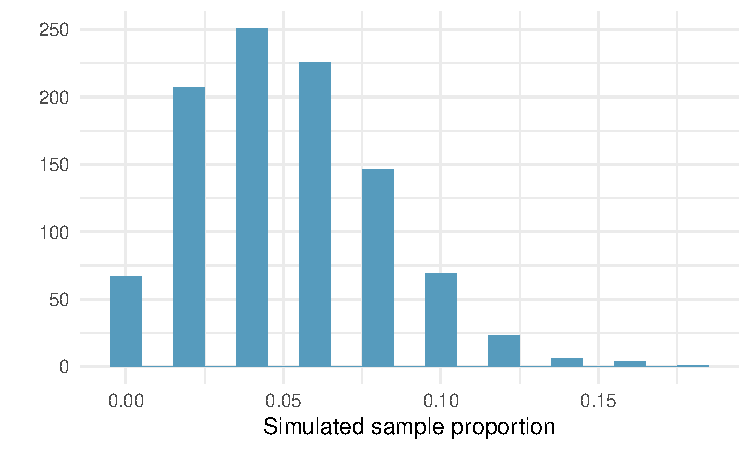
\includegraphics[width=0.55\textwidth]{\chp5@path/5-1_point_est_sampling_var/figures/sf/low-p.pdf}
\end{center}
}

\end{frame}

%%%%%%%%%%%%%%%%%%%%%%%%%%%%%%%%%%%

\begin{frame}

\dq{What happens when $np$ and/or $n(1-p)$ $<$ 10?}

\begin{center}
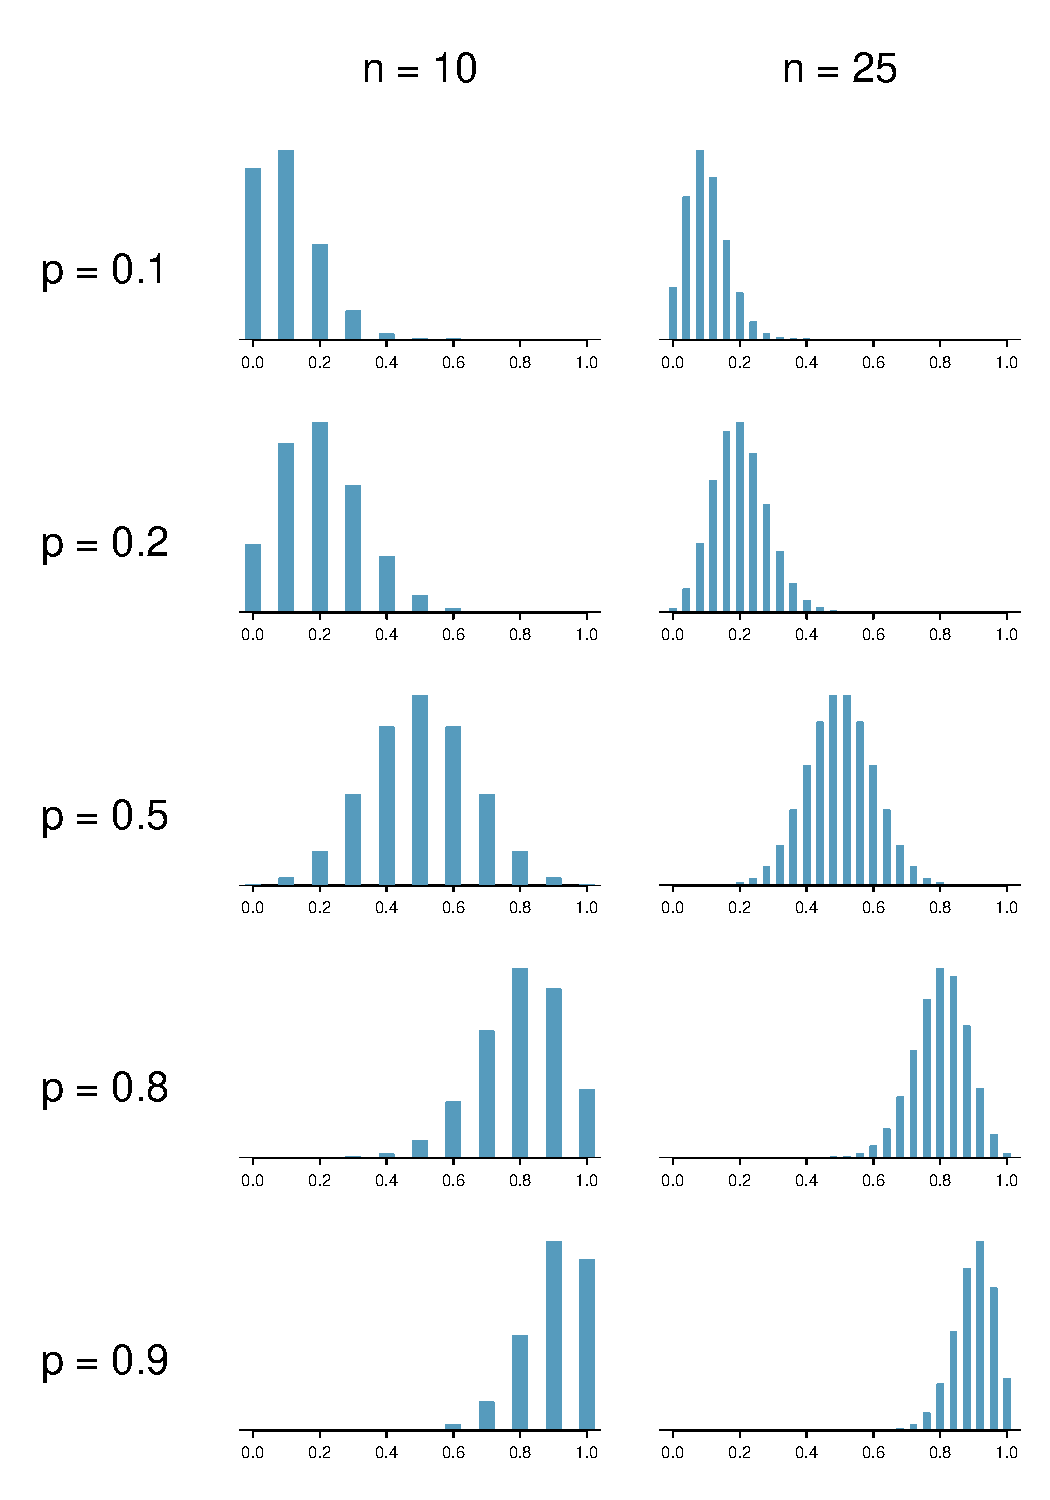
\includegraphics[width=0.45\textwidth]{\chp5@path/5-1_point_est_sampling_var/figures/clt_prop_grid/clt_prop_grid_1.pdf}
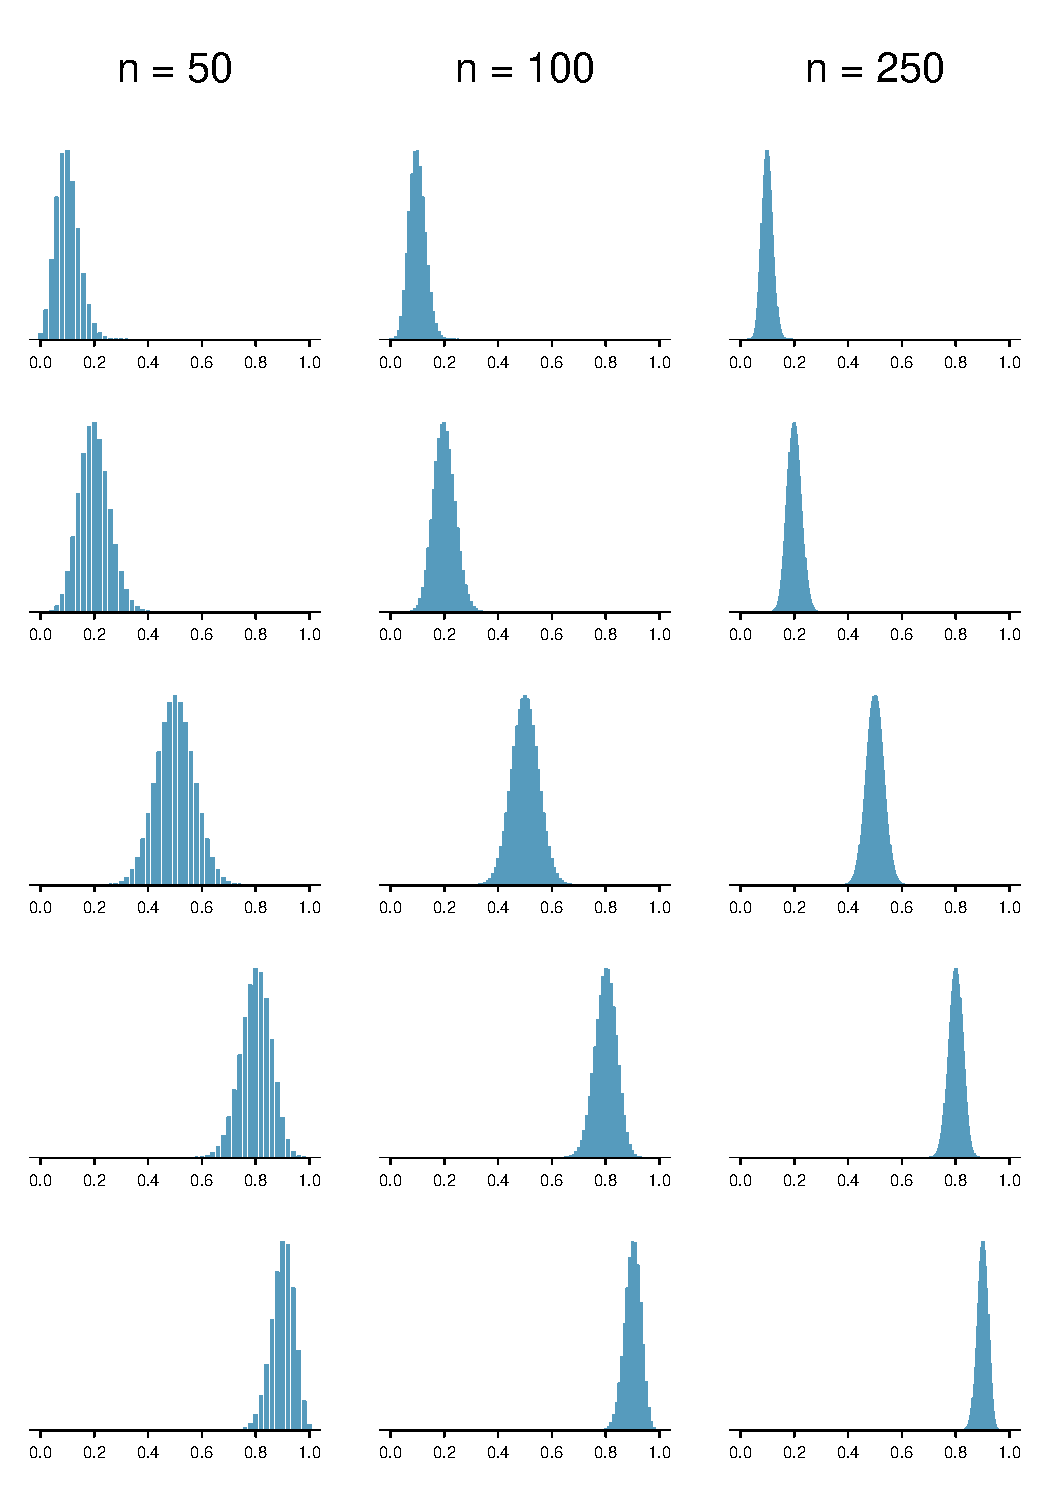
\includegraphics[width=0.45\textwidth]{\chp5@path/5-1_point_est_sampling_var/figures/clt_prop_grid/clt_prop_grid_2.pdf}
\end{center}

\end{frame}

%%%%%%%%%%%%%%%%%%%%%%%%%%%%%%%%%%%

\begin{frame}
\frametitle{When the conditions are not met...}

\begin{itemize}

\item When either $np$ or $n(1-p)$ is small, the distribution is more discrete.
\item When $np$ or $n(1-p)$ $<$ 10, the distribution is more skewed.
\item The larger both $np$ and $n(1-p)$, the more normal the distribution.
\item When $np$ and $n(1-p)$ are both very large, the discreteness of the distribution is hardly evident, and the distribution looks much more like a normal distribution.

\end{itemize}

\end{frame}

%%%%%%%%%%%%%%%%%%%%%%%%%%%%%%%%%%%%

\subsection{Extending the framework for other statistics}

%%%%%%%%%%%%%%%%%%%%%%%%%%%%%%%%%%%%

\begin{frame}
\frametitle{Extending the framework for other statistics}

\begin{itemize}

\item The strategy of using a sample statistic to estimate a parameter is quite common, and it's a strategy that we can apply to other statistics besides a proportion.

\begin{itemize}
\item Take a random sample of students at a college and ask them how many extracurricular activities they are involved in to estimate the average number of extra curricular activities all students in this college are interested in.
\end{itemize}

\item The principles and general ideas are from this chapter apply to other parameters as well, even if the details change a little. 

\end{itemize}

\end{frame}
